% Chapter 8

\chapter{Diseño del Protocolo CWC} % Chapter title

\label{ch:diseno_protocolo_cwc} % For referencing the chapter elsewhere, use \autoref{ch:name} 

%----------------------------------------------------------------------------------------

\section{Mensajes HTTP del Protocolo CWC}

\subsection{DGET}
Esta tal vez es una de los métodos de mayor importancia en el CWC, pues establece como obtener un archivo desde múltiples cachés. Este método se rige bajo el siguiente flujo:

\begin{enumerate}
\item Se verifica que el servidor web soporte el protocolo CWC.
\item Se solicita el top de miembros que tienen el archivo que se desea descargar. El número de miembros que se enviarán por petición se limitará a 100.
\item Se solicitan los atributos, Checksum y tamaño al servidor.
\item Si el tamaño del archivo es menor a 1MB, se solicita desde un solo miembro.
\item Si el tamaño del archivo es mayor a 1MB, se divide en segmentos y se asigna de la siguiente manera:

	\begin{enumerate}
	\item Al primer miembro del top se le asigna un equivalente al 10\% del tamaño del archivo en partes, si un 10\% es menor a un 1MB, se le asigna el tamaño correspondiente a 1MB.
	\item Al segundo se le asigna el equivalente a un 10\% del tamaño del archivo en partes, si un 10\% es menor a 1MB, se le asigna el tamaño correspondiente a 1MB. 
	\item Se realiza este procedimiento hasta llegar al quinto de la lista, después de esto se reparte equitativamente entre el resto de miembros.
	\item Si se da el caso de que el número de miembros es menor a 10, se reparte el total del archivo en partes iguales entre todos los miembros. 
	\end{enumerate}

\item Se inicia la descarga simultánea desde todos los miembros. En la figura \ref{DGET} se puede observar este proceso.

\item En el caso de que alguno de los miembros falle, se recurrirá al siguiente de mayor rango (mejor posicionado en el top) si se diera el caso de que no se tienen más miembros a quien recurrir se solicitaré el archivo o el segmento al servidor.

\item Cuando se ha terminado la descarga, se unen todas las partes y se envía el archivo al navegador web, como si el archivo fuera servido por un servidor web local.

\end{enumerate}

\begin{figure}
  \centering
    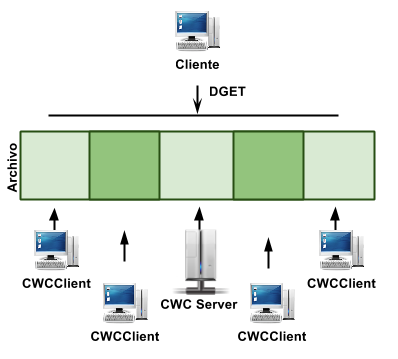
\includegraphics[scale=0.75]{gfx/DGET}
  \caption{Funcionamiento del DGET}
  \label{DGET}
\end{figure}


El DGET recibirá los siguientes parámetros:

\begin{enumerate}
\item Id del archivo.
\item Offset en partes.
\item Tamaño que debe leer.
\end{enumerate}

Por ejemplo, el archivo que se desea leer es el Id 10, y se debe leer a partir del byte 95, más los 50 bytes siguientes, entonces la llamada sería DGET(10, 95,50).

\subsection{DSEND}
Este es el caso contrario de DGET, es necesario recordar que un DGET tiene como parámetros el Id del archivo, el offset en partes y por último el tamaño que se debe leer en segmentos. Data esta información se puede enviar un flujo de segmentos hacia quien hizo el DGET.

\section{Estructura de los Mensajes CWC}
\label{sec:estructura_protocolo_cwc}

El protocolo de comunicación se basará en XML para realizar el envío y recepción de mensajes entre el servidor, los clientes y las cachés. En el presente apartado se definirá los mensajes que se intercambiarán y sus respuestas.

Cualquier mensaje que se envíe siempre tendrá tres componentes, que servirán como identificador de éste:

\begin{figure}[h]
  \centering
    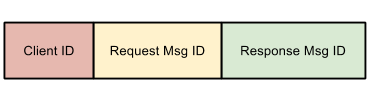
\includegraphics[scale=0.75]{gfx/EstructuraMensajeCWC}
  \caption{Estructura de un mensaje}
  \label{EstructuraMensajeCWC}
\end{figure}


En la figura \ref{EstructuraMensajeCWC} se observan los componentes del mensaje, los cuales son:

\begin{enumerate}
\item El identificador único del cliente en el sistema, este es generado cuando un cliente entra a formar parte de la comunidad, en el caso del servidor su identificador único es 0. En algunos mensajes se utilizará un identificador por defecto (-1) este significará que hay un nuevo cliente que desea convertirse en un miembro de la comunidad pero aun no tiene su identificador único.

\item Request Message Id: Este es el número del mensaje al que se esté respondiendo, cuando se encuentre el caso que no se esté respondiendo a ningún mensaje se introducirá un número negativo lo cual indicará que se está iniciando una comunicación.

\item Response Message Id: Este es el número del mensaje que estamos enviando, este número se genera como un aleatorio entre 1 y 10000, en algunos casos el mensaje no necesita respuesta entonces se introduce un número negativo.
\end{enumerate}

%------------------------------------------------

\section{Operaciones del Protocolo CWC}

En el presente apartado se definirán las operaciones necesarias para el funcionamiento del protocolo CWC. Aquí de detallará tanto valores de entrada, como de salida y además la estructura esperada. 

%------------------------------------------------

\subsection{ACK}

Este mensaje es una confirmación. Además puede ser enviado por cualquiera de las partes involucradas en la comunicación: Servidor o Cliente. Éste tiene la siguiente estructura mostrada en el listado \ref{lst:mensaje_ack}.

\begin{lstlisting}[language=XML,caption={Mensaje ACK},label={lst:mensaje_ack}]
<ack clientid="X" requestid="X" responseid="-1"> </ack>
\end{lstlisting}

\begin{description}
\item[Respuesta] No necesita respuesta.
\end{description}

%----------------------------------------------------------------------------------------

\subsection{GetClientId}

Este mensaje se utiliza cuando un nuevo CWCClient quiere formar parte de la comunidad. La estructura del mensaje se muestra en el listado \ref{lst:mensaje_getclientid}.

\begin{lstlisting}[language=XML,caption={Mensaje GetClientId},label={lst:mensaje_getclientid}]
<getClientId clientid="-1" requestid="-1" responseid="X"> 
</getClientId>
\end{lstlisting}


Como se puede observar el clientId es -1 ya que es un cliente nuevo, el requestId es -1 ya que no se está respondiendo a nadie y el responseid es un numero aleatorio entre 1 y 10000. 

\begin{description}
\item[Respuesta] La Respuesta esperada por parte del servidor se muestra en el listado \ref{lst:respuesta_getclientid}.
\end{description}

 \begin{lstlisting}[language=XML,caption={Mensaje de Respuesta GetClientId},label={lst:respuesta_getclientid}]
<getClientId clientid="0" requestid="X" responseid="Y"> 
	<client> Z </client>
</getClientId>
\end{lstlisting}

Para terminar la comunicación se espera por parte del cliente un ACK con su nuevo clientId.

\subsection{UpdateMembership}

Este mensaje se utiliza para establecer el tipo de membresía, recursos que se están prestando a la caché y tipo de administración. La primera vez que se utiliza, lo que se busca es crear la membresía, lo usos subsecuentes son básicamente para actualizar la información. La estructura del mensaje se muestra en el listado \ref{lst:mensaje_updatemembership}.

\begin{lstlisting}[language=XML,caption={Mensaje de UpdateMembership},label={lst:mensaje_updatemembership}]
<UpdateMembership clientid="X" requestid="-1" \\
		 responseid="Y"> 
	<type> Z </type>
	<manage> Z </manage>
	<disk> Z </disk>
	<mem> Z </mem>
	<upload> Z </upload>
</UpdateMembership>
\end{lstlisting}

Los valores que pueden tomar estas variables son:

\begin{itemize}
\item \textbf{type}: 1 = Voluntaria, 2 = Involuntaria
\item \textbf{manage}: 1 = Atendida, 2 = desatendida, 3 = Administrada por servidor
\item \textbf{disk}: En MB un número mayor o igual a 100
\item \textbf{mem}: En MB un número mayor o igual a 100
\item \textbf{upload}: En KB un número mayor o igual 128
\end{itemize}

\begin{description}
\item[Respuesta] Se espera como respuesta un ACK por parte del servidor.
\end{description}

\subsection{GetObjectInfo}
Este mensaje se utiliza para obtener la información de un objeto cachéable. La estructura del mensaje se muestra en el listado \ref{lst:mensaje_getobjectinfo}.

\begin{lstlisting}[language=XML,caption={Mensaje de GetObjectInfo},label={lst:mensaje_getobjectinfo}]
<GetObjectInfo clientid="X" requestid="-1" responseid="Y"> 
	<objectId> Z </objectId>
	<objectLocation> Z </objectLocation>
</GetObjectInfo>
\end{lstlisting}

Los valores que pueden tomar estas variables son:

\begin{itemize}
\item \textbf{objectId}: El identificador único del objeto.
\item \textbf{objectLocation}: El URI relativo del objeto cachéable.
\end{itemize}

Es posible que se incluya solo uno o ambos.

\begin{description}
\item[Respuesta] La Respuesta esperada por parte del servidor se muestra en el listado \ref{lst:respuesta_getobjectinfo}.
\end{description}

\begin{lstlisting}[language=XML,caption={Mensaje de Respuesta de GetObjectInfo},label={lst:respuesta_getobjectinfo}]
<response clientid="0" requestid="X" responseid="Y"> 
	<checksum> Z </checksum>
	<id> Z </id>
	<location> Z </location>
	<size> Z </size>
	<expdate> Z </expdate>
</response>
\end{lstlisting}

Lo valores que retorna son:

\begin{itemize}
\item \textbf{checksum}:  El Checksum del archivo
\item \textbf{id}: El identificador del objeto
\item \textbf{location}: URI relativo donde se encuentra el objeto.
\item \textbf{size}: Tamaño del archivo en megabytes
\item \textbf{expdate}: Fecha de expiración.
\end{itemize}


La respuesta esperada por parte del cliente es un ACK.

\subsection{ModifyObject}
Este mensaje es enviado por el servidor, en este caso se ha realizado un cambio del lado del servidor que debe ser propagado hacia los clientes. La estructura del mensaje se muestra en el listado \ref{lst:mensaje_modifyobject}.

\begin{lstlisting}[language=XML,caption={Mensaje de ModifyObject},label={lst:mensaje_modifyobject}]
<ModifyObject clientid="0" requestid="X" responseid="Y"> 
	<checksum> Z </checksum>
	<id> Z </id>
	<location> Z </location>
	<size> Z </size>
	<expdate> Z </expdate>
	<type> Z </type>
</ModifyObject>
\end{lstlisting}

La única diferencia con el anterior es el type, el cual especifica el tipo de modificación que se está realizando, 1 significa una modificación soft la cual no necesita actualizar el archivo y cualquier otra cosa es una modificación hard lo que implica que hay que deshabilitar el archivo y volverlo a cargar.

\begin{description}
\item[Respuesta] La respuesta esperada por parte del cliente es un ACK.
\end{description}

\subsection{Enable-Disable Object}

En este caso el mensaje se utiliza para habilitar o deshabilitar un objeto que se encuentra en la caché. Este mensaje puede ser enviado tanto por el servidor como por el cliente. La estructura del mensaje se muestra en el listado \ref{lst:mensaje_enableobject}.

\begin{lstlisting}[language=XML,caption={Mensaje de EnableObject},label={lst:mensaje_enableobject}]
<EnableObject clientid="X" requestid="-1" responseid="Y"> 
	<objectId> Z </objectId>
</EnableObject>
\end{lstlisting}

Se envía el identificador del objeto, si el objeto esta Enable se cambia a Disable o viceversa  y se espera un ACK de parte de la otra parte.

\begin{description}
\item[Respuesta] La respuesta esperada por parte del cliente o servidor, según corresponda, es un ACK.
\end{description}

\subsection{DeleteObject}
Este mensaje es utilizado ya sea por los clientes o por el servidor, cuando un objeto se borra en alguno de los dos. La estructura del mensaje se muestra en el listado \ref{lst:mensaje_deleteobject}.

\begin{lstlisting}[language=XML,caption={Mensaje de DeleteObject},label={lst:mensaje_deleteobject}]
<DeleteObject clientid="X" requestid="-1" responseid="Y"> 
	<objectId> Z </objectId>
</DeleteObject>
\end{lstlisting}

Se envía el identificador del objeto y se registra el borrado, en el caso del cliente borra el objeto de la caché, en el caso del servidor borra la relación entre la caché y el objeto.

\begin{description}
\item[Respuesta] La respuesta esperada por parte del cliente o servidor, según corresponda, es un ACK.
\end{description}

\subsection{GetMemberStatus}
\label{GetMemberStatus} 
Este mensaje es utilizado para solicitar el estado de un miembro de la caché (no del servidor), se puede ejecutar tanto por el servidor como por cualquier miembro de la caché. La estructura del mensaje se muestra en el listado \ref{lst:mensaje_getmemberstatus}.

\begin{lstlisting}[language=XML,caption={Mensaje de GetMemberStatus},label={lst:mensaje_getmemberstatus}]
<GetMemberStatus clientid="X" requestid="-1" responseid="Y"> 
	<memberId> Z </memberId>
</GetMemberStatus>
\end{lstlisting}

\begin{description}
\item[Respuesta] Se envía el memberId que es igual al clientId, se espera la respuesta mostrada en el listado \ref{lst:respuesta_getmemberstatus}.
\end{description}

\begin{lstlisting}[language=XML,caption={Mensaje de Respuesta de GetMemberStatus},label={lst:respuesta_getmemberstatus}]
<response clientid="0" requestid="X" responseid="Y"> 
	<status> Z </status>
</response>
\end{lstlisting}

El status puede tomar los siguientes valores 0 = desconocido, 1 = activo, 2 = no-activo, 3 = offline y 4 = online.

Se espera un ACK por parte de quien solicitó el status.

\subsection{ChangeMemberStatus}
Este mensaje es utilizado para cambiar el status de un miembro de la caché, este solo puede ser ejecutado por parte del servidor hacia cualquiera de los clientes o  por parte del cliente hacia el servidor para cambiar su estatus. La estructura del mensaje se muestra en el listado \ref{lst:mensaje_changememberstatus}.

\begin{lstlisting}[language=XML,caption={Mensaje de ChangeMemberStatus},label={lst:mensaje_changememberstatus}]
<ChangeMemberStatus clientid="0" requestid="X" \\
		 responseid="Y"> 
	<memberId> Z </memberId>
	<status> Z </status>
</ChangeMemberStatus>
\end{lstlisting}


El status puede tomar cualquier valor de la operación definida en \ref{GetMemberStatus}. 


\begin{description}
\item[Respuesta] La respuesta esperada por parte del cliente es un ACK.
\end{description}

\subsection{GetListOfFiles}

Este mensaje se utiliza ya sea para pedir una lista de archivos a un cliente con su respectivo checksum o para solicitar una lista de archivo que debería tener un cliente en su caché con su respectivo checksum. La estructura del mensaje se muestra en el listado \ref{lst:mensaje_getlistoffiles}.

\begin{lstlisting}[language=XML,caption={Mensaje de GetListOfFiles},label={lst:mensaje_getlistoffiles}]
<GetListOfFiles clientid="0" requestid="X" responseid="Y"> 
	<clientId> Z </clientId>
</GetListOfFiles>
\end{lstlisting}

\begin{description}
\item[Respuesta] La Respuesta esperada por parte del cliente se muestra en el listado \ref{lst:respuesta_getlistoffiles}.
\end{description}

\begin{lstlisting}[language=XML,caption={Mensaje de Respuesta de GetListOfFiles},label={lst:respuesta_getlistoffiles}]
<response clientid="0" requestid="X" responseid="Y"> 
	<file objectId="Z" checksum="Z"> </file>
	<file objectId="Z" checksum="Z"> </file>
	<file objectId="Z" checksum="Z"> </file>
</response>
\end{lstlisting}

Se espera un ACK por parte de quien recibe la lista de archivos.

\subsection{GetStats}
Se ejecuta por parte del servidor, para obtener las estadísticas de una de las cachés. La estructura del mensaje se muestra en el listado \ref{lst:mensaje_getstats}.

\begin{lstlisting}[language=XML,caption={Mensaje de GetStats},label={lst:mensaje_getstats}]
<GetStats clientid="X" requestid="-1" responseid="Y"> 
	<clientId> Z </clientId>
</GetStats>
\end{lstlisting}



\begin{description}
\item[Respuesta] La Respuesta esperada por parte del cliente se muestra en el listado \ref{lst:respuesta_getstats}.
\end{description}

\begin{lstlisting}[language=XML,caption={Mensaje de Respuesta de GetStats},label={lst:respuesta_getstats}]
<response clientid="0" requestid="X" responseid="Y"> 
	<maxupload> Z </maxupload>
	<minupload> Z </minupload>
	<maxclients> Z </maxclients>
	<currentclients> Z </currentclients>
</response>
\end{lstlisting}

Se envía la máxima velocidad de transferencia, la mínima velocidad de trasferencia, máxima cantidad de clientes simultaneemos y clientes actuales.

Se espera un ACK por parte de quien recibe las estadísticas.

\subsection{SendStats}

En algunos casos las estadísticas son enviadas por el mismo cliente, en este caso la estructura del mensaje se muestra en el listado \ref{lst:mensaje_sendstats}.

\begin{lstlisting}[language=XML,caption={Mensaje de SendStats},label={lst:mensaje_sendstats}]
<SendStats clientid="0" requestid="X" responseid="Y"> 
	<maxupload> Z </maxupload>
	<minupload> Z </minupload>
	<maxclients> Z </maxclients>
	<currentclients> Z </currentclients>
</SendStats>
\end{lstlisting}

\begin{description}
\item[Respuesta] La Respuesta esperada por parte del servidor es un ACK.
\end{description}

\subsection{GetTopCachesbyObject}

Este mensaje es enviado por los clientes, para solicitar el top de cachés que pueden servir un objeto. El formato del mensaje se muestra en el listado \ref{lst:mensaje_gettopcaches}.

\begin{lstlisting}[language=XML,caption={Mensaje de GetTopCachesbyObject},label={lst:mensaje_gettopcaches}]
<GetTopCachesbyObject clientid="0" requestid="X" \\
		 responseid="Y"> 
	<objectId> Z </objectId>
</GetTopCachesbyObject>
\end{lstlisting}


\begin{description}
\item[Respuesta] La Respuesta esperada por parte del servidor se muestra en el listado \ref{lst:respuesta_gettopcaches}.
\end{description}

\begin{lstlisting}[language=XML,caption={Mensaje de Respuesta de GetTopCachesbyObject},label={lst:respuesta_gettopcaches}]
<response clientid="0" requestid="X" responseid="Y"> 
	<cache clientId="Z" URL="Z"> </cache>
	<cache clientId="Z" URL="Z"> </cache>
	<cache clientId="Z" URL="Z"> </cache>
</response>
\end{lstlisting}


Se espera un ACK por parte del cliente que recibió esta lista.

\subsection{GetConfParams}
Este también es únicamente ejecutado por el cliente, se utiliza para tomar la configuración del sistema, hay varios parámetros que pueden cambiar, este mensaje se utiliza para obtener estos cambios. La estructura del mensaje se muestra en el listado \ref{lst:mensaje_getconfparams}.

\begin{lstlisting}[language=XML,caption={Mensaje de GetConfParams},label={lst:mensaje_getconfparams}]
<GetConfParams clientid="0" requestid="X" responseid="Y"> 
</GetConfParams>
\end{lstlisting}


\begin{description}
\item[Respuesta] La Respuesta esperada por parte del servidor se muestra en el listado \ref{lst:respuesta_getconfparams}.
\end{description}

\begin{lstlisting}[language=XML,caption={Mensaje de Respuesta de GetConfParams},label={lst:respuesta_getconfparams}]
<response clientid="0" requestid="X" responseid="Y"> 
	<param paramId="Z"> </param>
	<param paramId="Z"> </param>
	<param paramId="Z"> </param>
</response>
\end{lstlisting}


Se espera un ACK por parte de quien recibe la lista de parámetros.

\subsection{IsAlive}

Este mensaje se utiliza para saber si algún miembro del sistema está vivo. La estructura del mensaje se muestra en el listado \ref{lst:mensaje_isalive}.

\begin{lstlisting}[language=XML,caption={Mensaje de IsAlive},label={lst:mensaje_isalive}]
<IsAlive clientid="X" requestid="-1" responseid="Y"> 
</IsAlive>
\end{lstlisting}

\begin{description}
\item[Respuesta] Para este mensaje es espera un ACK por parte de la caché representada por clientId.
\end{description}

\section{Seguimiento de los miembros conectados}

Es de suma importancia saber si alguno de los miembros de la CWC se encuentra bien, para esto se deberá estar revisando que los miembros estén en línea, para lograrlo, se seguirá:

\begin{enumerate}
\item El servidor tendrá una estampa de tiempo para cada caché, la cual indicará la última vez que se recibió un mensaje por parte de ésta.
\item Cada caché tendrá una estampa de tiempo del servidor que indicará la última vez que este envió un mensaje.
\item Existirá un parámetro configurable llamado "tiempo sin respuesta", el cual establece cuanto tiempo debe pasar después de que se recibió un mensaje para preocuparse.
\item Cada vez que se recibe un mensaje por parte de alguna caché o el servidor, se establece esta estampa a la hora en la cual se recibió el mensaje.
\item Se estará revisando periódicamente si alguna estampa ya es lo suficientemente antigua como para que el tiempo actual menos la estampa del último mensaje se mayor o igual al "tiempo sin respuesta".
\item Si ha pasado más tiempo del establecido por "tiempo sin respuesta", se envía un mensaje de IsAlive.
\item Si no se recibe respuesta después de tres intentos se establece que esa caché o servidor esta caído.
\item En el caso de una caché, se seguirá revisando periódicamente en tiempos no menores a "tiempo sin respuesta" hasta que se descubra que está arriba.
\item En el caso del servidor se actualizará la caché como offline y se esperaré a que ésta se comunique.
\end{enumerate}

\section{Recuperación de fallas}
Cuando se presenta una falla, se puede dar ya sea en el lado del servidor como del lado de alguno de los clientes, el protocolo que se seguirá es:

\subsection{¿Cómo descubrir una falla?}
Para descubrir una falla se deben de dar las siguientes condiciones:
\begin{enumerate}
\item En el caso del servidor perder contacto con todas las cachés y con Internet (una implica a la otra).
\item En el caso de un cliente perder la conexión con el servidor o con Internet (una implica a la otra). 
\end{enumerate}

\subsection{Falla del Servidor}
Una falla se puede dar por muchas razones, no es el objetivo de este proyecto estudiarlas, pero en cualquier caso se pueden clasificar en dos tipos:

\begin{itemize}
\item Perder información volátil: Esto quiere decir que el servidor, por ejemplo se apaga. Esta acción produce que la información que estaba en memoria y no se había enviado a disco, o a base de datos mediante un flush, se pierda.
\item Información volátil intacta: Por ejemplo, se pierde la conexión a Internet o se apaga voluntariamente el servidor, por consiguiente se cortan las funciones de red.
\end{itemize}

En cualquiera de los casos anteriormente mencionados, este es el protocolo ejecuta el algoritmo definido a continuación:

\begin{enumerate}
\item Si es sin pérdida de información volátil: Se debe hacer un flush inmediatamente.
\item Una vez que se haya recuperado de la falla, la detección consiste en comprobar que existe comunicación entre las cachés e Internet, se establecen todas las caché en un estado inactivo.
\item Cargar la información a memoria.
\item Esperar a la petición por estado, cuando el estado es inactivo se procede a revisar la consistencia.
\item Esperar a recibir los mensajes por parte de las cachés, que ante esta eventualidad, enviarán mensajes GetListOfFiles.
\item Esperar hasta que las cachés envíen un cambio (ChangeStatus) de estado a: en línea.
\item Esperar que se repita las veces que sean necesarias.
\item Después que las cachés se encuentren en línea, se retomarán los mensajes donde habían quedado (es necesario recordar, que en el caso que el último mensaje enviado, no se haya recibido respuesta, se declara que el servidor está fuera de línea hasta que éste responda y se retoma la comunicación en el último mensaje enviado).
\end{enumerate}

\subsection{Falla un Cliente}
En este caso, la caché por alguna razón perdió comunicación y el servidor la marcó como inactiva. Cuando se recupera la comunicación, lo primero que se solicita es el estado de la caché. Éste recibirá un mensaje de desactivación, por lo que pedirá los archivos para revisar la consistencia. Cuando todo esté correcto, se solicitará volver al estado \textit{en línea} y seguirá la comunicación como se encontraba anteriormente.
Para reconstruir el DGET, el cliente deberá evaluar la cantidad de partes descargadas y solicitar la lista de cachés disponibles al servidor para retomar la descarga.

\section{Implementación del Modelo de Consistencia}
Como se mencionó anteriormente, el modelo de consistencia no es tan complejo, debido a que solo un actor es el que modifica los objetos que se incluyen en la caché, este actor es el CWCServer. El modelo de consistencia bastará con:

\begin{itemize}
\item Si se modifica un objeto en el servidor, este ejecutará un ModifyObject hacia todas las cachés que tienen copias de este objeto, si es un cambio de archivo tamaño, entre otros. Decidirá si es necesario eliminar el archivo y volver a solicitarlo.
\item Las cachés estarán revisando periódicamente, la consistencia, esto quiere decir que solicitará al servidor el Checksum de los archivos que tiene en su caché, lo calculará y lo comparará.
\item Si hay algo extraño, simplemente solicita que se envíe el archivo de nuevo, si todo está bien pues no hay ningún problema.
\item Después de una falla se revisa la consistencia, esto aplica para todas las cachés en el caso de que sea una falla de servidor o para la caché que fallo.
\end{itemize}